%Paul E. West and Sean T. Hayes

\documentclass[14pt,aspectratio=1610, hyperref={pdfpagelayout=SinglePage}]{beamer}
% \documentclass[14pt,aspectratio=1610, hyperref={pdfpagelayout=SinglePage}, handout]{beamer}
\usepackage{csu-theme}
\usepackage{booktabs}

\usepackage{tikz}
\usepackage{gnuplot-lua-tikz}
\usepackage{gnuplottex}
% \usetikzlibrary{arrows,patterns,plotmarks,backgrounds,fit}
% \input gnuplot-lua-tikz-common.tex
% \endinput

\title{\Huge{}Performance\\ Analysis}
\subtitle{CSCI 315: \textit{Data Structure Analysis}\\Chapter 18}
%\author{Sean T. Hayes, PhD}
\institute{Charleston Southern University}

%% Comment out date to use default (today)
% \date{February 4, 2025}
\subject{Software Programming}
%\keywords{Performance Counters, Multicore}

\graphicspath{{../imgs/performance}}

\begin{document}

\begin{frame}
  \titlepage{}
\end{frame}

\section{Intro}

\begin{frame}{Analysis of Algorithms}
  \emph{Dilemma}: You have two (or more) solutions to a\\ problem.\\
  How do you choose the BEST method?
\begin{itemize}
\item<2->
  One approach: Implement each algorithm in C++;\\ test how long each takes to run.
\item<3->
  Problems:
  \begin{itemize}
  \item<3->
    Different implementations may cause an algorithm to run faster/slower.
  \item<4->
    Some algorithms run faster on some computers.
  \item<5->
    Algorithms may perform differently depending on data (e.g., sorting often
    depends on what is being sorted).
  \end{itemize}
\end{itemize}
\end{frame}

\begin{frame}{A Fundamental Computer Science Challenge}
\begin{itemize}[<+->]
\item
  One of the most fundamental tools for computer scientists to analyze the \emph{cost} of an
algorithm.\\[1em]
\item
  The cost can be described in terms of time, space (memory usage), electricity, etc.\\[1em]
\item
  Ideally, we will develop a simple scheme to rank algorithms from best to worst.
\end{itemize}
\end{frame}

\begin{frame}{Approaches to Analyzing Performance}
  Two approaches to describing ``general'' algorithm performance:
  \begin{enumerate}
  \item<2->
    \textbf{Empirical (Experimental)}: Measure performance for examples.\\ But, what does this tell us in general?
  \item<3->
    \textbf{Analytical (Asymptotic)}:
    \begin{itemize}
    \item<4-> Assess performance in an abstract, generalized manner.
    \item<5-> Idea: analyze performance as the size of problem growth.
    \item<6-> Examples:
    \begin{itemize}
    \item Sorting: How many comparisons for an array of size \(n\)?
    \item Searching: How many comparisons for an array of size \(n\)?
    \end{itemize}
    \item<7-> Challenge: It may be difficult to discover a reasonable formula.
    \end{itemize}
  \end{enumerate}
\end{frame}


\begin{frame}{Analytical Approach}

Characterize performance by counting the number of\\ operations.

\begin{itemize}
\item <2->
  \emph{Sorting}: the operations include when:
  \begin{itemize}
  \item
    two values are compared and
  \item
    two values are swapped.
  \end{itemize}
\item <3->
  \emph{Search}:
  \begin{itemize}
  \item
    Count the number of times the value being searched for is compared to values in an array.
  \end{itemize}
\item <4->
  \emph{Recursion}:
  \begin{itemize}
  \item
    Count the number of recursive calls.
  \end{itemize}
\end{itemize}

\onslide<5->{
However, the number of operations is dependent on \\the size and characteristics of the data.}

\end{frame}

\begin{frame}{Analysis with Varying Results}
\begin{itemize}
\item
  Example: some sorting algorithms may require\\ as few as \(n-1\) comparisons and as many as \(\frac{1}{2}n^2\).
\item<2->
  Types of analyses based a problem of size \(n\):
  \begin{itemize}
  \item
    \emph{Best} case: What is the shortest an algorithm can run?
  \item
    \emph{Average} case: On average, how fast does an algorithm run?
  \item
    \emph{Worst} case: What is the longest an algorithm can run?
  \end{itemize}
\item<3->
  Computer scientists \textit{usually} use worst-case or average-case analysis.
  \end{itemize}
\end{frame}

\begin{frame}{Worst Case vs. Average Case}
  \centering\large
What are some examples of domains where you may care more about the \emph{worst case} than the \emph{average case} and vice versa?
\end{frame}

\begin{frame}{Notice: We Are \textbf{Approximating}}
\begin{itemize}
\item We usually \emph{approximate} the an algorithm's performance, assuming it is operating on a very large data set.
\item Approximating is an important skill to learn and use.
\end{itemize}
\end{frame}

\begin{frame}{Simpler Question: How many hotdogs\\ tall is the Empire State Building?}
\begin{columns}
\column{0.670\textwidth}
\begin{itemize}
\item<2-> The ESB is \(1,250\) feet tall.
\item<3-> Assuming that a hotdog is 6 inches from end to end, you would need, \(1,250 \cdot 2 = 2,500\) hotdogs.
\end{itemize}
\column{0.33\textwidth}
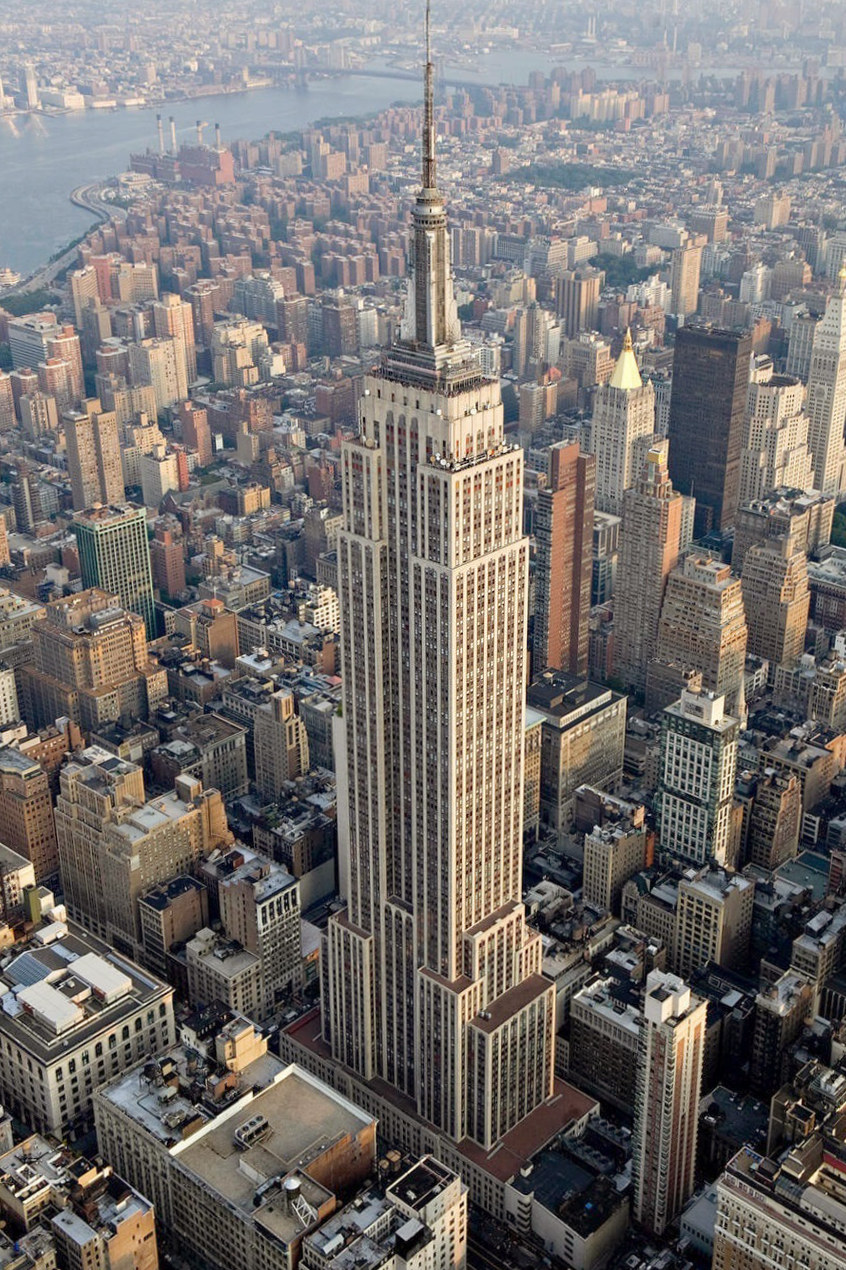
\includegraphics[width=0.8\textwidth]{empire-state-building}
\end{columns}
\end{frame}


\section{Complexity Analysis}

\begin{frame}{Analysis}
\begin{itemize}[<+->]
\item Utilize an objective way to evaluate the \emph{cost} of an\\ algorithm or code section.
\item The cost is usually computed in terms of \emph{time} or \emph{space}.
\item The goal is to have a meaningful way to compare algorithms based on a common measure.
% \item Complexity analysis has two phases,
%   \begin{enumerate}
%   \item Algorithm analysis
%   \item Complexity analysis
%   \end{enumerate}
\end{itemize}
\end{frame}


\begin{frame}{Algorithm Analysis}
\begin{itemize}[<+->]
\item Algorithm analysis requires a set of rules to determine how operations are to be counted.
\item There is no generally accepted set of rules for algorithm analysis.
\item In some cases, an exact count of operations is desired; in other cases, a general approximation is sufficient.
\item The following rules are typical of those intended to exactly count operations.
\end{itemize}
\end{frame}


\begin{frame}{Rules for Estimation}
\begin{enumerate}
\item We \emph{assume} an arbitrary time unit.
\item Execution of one of the following operations takes time 1:
  \begin{itemize}
  \item assignment operation
  \item single I/O operations
  \item single Boolean operations, numeric comparisons
  \item single arithmetic operations
  \item function return
  \item array index operations, pointer dereferences
  \end{itemize}
\end{enumerate}
\end{frame}

\begin{frame}[fragile]{Example 1}
\begin{lstlisting}[mathescape]
count = count + 1;  // Cost: $\color{codeComment}c_1$
sum = sum + count;  // Cost: $\color{codeComment}c_2$ 
\end{lstlisting}
\vspace{2em}
\emph{Total Cost} \(= c_1 + c_2\). \\[1em]
Because we assume the addition costs 1 and assignment costs 1, the total cost is 4 units.
\end{frame}

\begin{frame}[fragile]{Conditional Cost}
\begin{lstlisting}[mathescape]
if (n < 0) {     // Cost: $\color{codeComment}c_1 \onslide<2->{= 1}$
    absVal = -n; // Cost: $\color{codeComment}c_2 \onslide<3->{= 2}$
} else {
    absVal = n;  // Cost: $\color{codeComment}c_3 \onslide<4->{= 1}$
}
\end{lstlisting}
\begin{itemize}[<+->]
\item
  \(\mathrm{Total Cost} \le c_1 + \max(c_2, c_3)\)
\item \(c_1\) is the cost of the boolean evaluation (\(1\) instruction).
\item \(c_2\) is the cost of the negating a number (\(1\)) + the cost of assignment (\(1\)).
\item \(c_3\) is the cost of an assignment (\(1\)).
\item
  \begin{tabular}{ccc}
    Worse Case & Best Cast & Average\\
    \(3\) & \(2\) & \(2.5\)
  \end{tabular}
\end{itemize}
\end{frame}

\begin{frame}[fragile]{Example 3}
\begin{lstlisting}[mathescape]
i = 1;             // Cost: $\color{codeComment}c_1\onslide<2->{= 1}$
sum = 0;           // Cost: $\color{codeComment}c_2\onslide<3->{= 1}$
while (i <= n) {   // Cost: $\color{codeComment}c_3\onslide<4->{= 1}$
    i = i + 1;     // Cost: $\color{codeComment}c_4\onslide<5->{= 1 + 1 = 2}$
    sum = sum + i; // Cost: $\color{codeComment}c_5\onslide<6->{= 2}$
}
\end{lstlisting}
\begin{itemize}
\item<5-> Remember assignment (\lstinline{=}) and addition (\lstinline{+}) each cost \(1\).
\item<7-> How many times does the loop execute?\\
  \onslide<8->{\(n\) times.}
\item<9-> \(\mathrm{Total Cost} = c_1 + c_2 + (n+1) c_3 + n \left(c_4 + c_5\right) =\) \\
\(c_1 + c_2 + c_3 + n\left(c_3 + c_4 + c_5\right)\)
\end{itemize}
\end{frame}

\begin{frame}{More Rules for Estimation}
\begin{enumerate}[<+->]
\setcounter{enumi}{2}
\item
  \emph{Selection statement} (if, switch) time is the time for the condition evaluation, plus the maximum of the running times for the individual clauses in the selection.
\item
  \emph{Loop execution} time is the number or iterations multiplied by its body's execution time, plus the time for the loop check and update operations, plus the loop setup time.\\
  Always assume that the loop iterates the maximum number of times.
\item
  The runtime of a \emph{function call} is 1 for setup plus the time for any parameter calculations plus the time required for the execution of the function body.
\end{enumerate}
\end{frame}

\begin{frame}[fragile]{Nested Example}
\begin{columns}[t]
\column{0.35\textwidth}
\begin{lstlisting}[basicstyle=\footnotesize\ttfamily]
i = 1;
sum = 0;
while (i <= n) {
    j = 1;
    while (j <= n) {
        sum += i;
        ++j;
    }
    ++i;
}
\end{lstlisting}
\column{0.1\textwidth}
{\footnotesize
\textbf{Cost}\\[6pt]
\(c_1 = 1\)\\
\(c_2 = 1\)\\
\(c_3 = 1\)\\
\(c_4 = 1\)\\
\(c_5 = 1\)\\
\(c_6 = 2\)\\
\(c_7 = 2\)\\
~\\
\(c_8 = 2\)
}
% \begin{lstlisting}[basicstyle=\footnotesize\ttfamily,language={},numbers=none,keepspaces=true]
% Cost
% c1 = 1
% c2 = 1
% c3 = 1
% c4 = 1
% c5 = 1
% c6 = 2
% c7 = 2

% c8 = 2


% \end{lstlisting}

\column{0.5\textwidth}
\begin{itemize}
\item <2-> The outer loop iterates \(n\) times.
\item <3-> For each iteration of the outer loop, the inner loop iterates \(n\) times.
\item <4-> The total cost is:\vspace{-1em}
  {\small
  \begin{align*}
  & c_1 + c_2 + n \left( c_4 + n \left( c_5 + c_6 + c_7 \right) + c_8 \right)\\
  = & c_1 + c_2 + n \left(c_4 + c_8\right) + n^2 \left( c_5 + c_6 + c_7 \right)\\
  = & 2 + 3n + 5n^2
  \end{align*}}
\end{itemize}
\end{columns}
\vspace{-0.5em}
\onslide<5->{\centerline{\textbf{Important Note:} \(n^2\) is the highest (largest) term!}}
\end{frame}

\section{Big \textit{O} Notation}
% A Notation for Complexity Analysis

\begin{frame}{Comparing Algorithms}
  \begin{itemize}[<+->]
  \item An algorithm's time requirement is a function of the problem size.
  \item The problem size depends on the application (e.g., the number of list elements for a sorting algorithm). % , the number of disks for the \href{https://en.wikipedia.org/wiki/Tower_of_Hanoi}{Towers of Hanoi}
  \item For instance, we say that (if the problem size is \(n\))
  \begin{itemize}
    \item Algorithm A requires \(5n^2\) time units to solve a problem of size \(n\).
    \item Algorithm B requires \(7n + 100\)  time units to solve a problem of size \(n\).
  \end{itemize}
  \end{itemize}
\end{frame}

\begin{frame}{Comparing Algorithms}
  \begin{itemize}[<+->]
    \item An algorithm's proportional time requirement\\ is known as the \emph{growth rate}.
    \item We can compare the efficiency of algorithms by comparing their growth rates.
  \end{itemize}
\end{frame}

\begin{frame}[fragile]{Comparing Algorithms}
\setbeamercolor{block body}{bg=white, fg=black}

%\begin{block}{}
\input plots/07-performance-analysis/performance-growth-rate1.tex
% \centerline{
\includegraphics[width=0.8\textwidth]{performance-growth-rate1}}
%\end{block}

\end{frame}

\begin{frame}{Example: Which is faster?}
% \begin{columns}
% \column{0.45\textwidth}\(50n^2 + 31n^3 + 24n + 15\)
% \column{0.5\textwidth}\(3n^2 + n + 21 + 4 \cdot 3^n\)
% \end{columns}
% \pause{}
%\centering
\onslide<2->{It depends on \(n\).}\\
\begin{tabular}{r @{\hskip 0.75cm} r @{\hskip 1cm} r}
\toprule{}
  \uncover<3->{\(n\)}  & \(50n^2 + 31n^3 + 24n + 15\) & \( 4 \cdot 3^n + 3n^2 + n + 21 \) \\
\midrule{}
  \onslide<3->{  1   &        120     &            37 }\\
  \onslide<3->{  2   &        511     &            71 \\}
  \onslide<3->{  3   &      1,374     &           159 \\}
  \onslide<3->{  4   &      2,895     &           397 \\}
  \onslide<3->{  5   &      5,260     &         1,073 \\}
  \onslide<3->{  6   &      8,655     &         3,051 \\}
  \onslide<3->{  7   &     13,266     &         8,923 \\}
  \onslide<3->{  8   &     19,279     &        26,465 \\}
  \onslide<3->{  9   &     26,880     &        79,005 \\}
  \onslide<3->{ 10   &     36,255     &       236,527} \\
\bottomrule{}
\end{tabular}

\end{frame}

\begin{frame}[t]{One term dominated the others.}
%\begin{center}
\onslide<2->{
  \begin{tabular}{r @{\hskip 0.75cm} r r c }
    \toprule{}
    \(n\)  & \( 4 \cdot 3^n + 3n^2 + n + 21\)  & \(4 \cdot 3^n\) & Proportion \\
    \midrule{}
    1  &          37  &         12  &      32.4\% \\
    2  &          71  &         36  &      50.7\% \\
    3  &         159  &        108  &      67.9\% \\
    4  &         397  &        324  &      81.6\% \\
    5  &       1,073  &        972  &      90.6\% \\
    \vdots{}  & \vdots{} & \vdots{} &   \vdots{}  \\
    % 6  &       3,051  &      2,916  &      95.6\% \\
    % 7  &       8,923  &      8,748  &      98.0\% \\
    % 8  &      26,465  &     26,244  &      99.2\% \\
    9  &      79,005  &     78,732  &      99.7\% \\
    10 &     236,527  &    236,196  &      99.9\% \\
    \bottomrule{}
  \end{tabular}
}

\onslide<3->{We only care about the highest-order (dominating) term.}
%\end{center}

\end{frame}

\begin{frame}{As \(n\) Grows, Some Terms Dominate}

\begin{tabular}{r r r r r r}
  \toprule{}
      \(n\)      & \(10\)   & \(100\)  & \(1,000\) & \(10,000\) & \(100,000\) \\
  \midrule{}
\(n^0\) or \(1\)  & \(k\)      & \(k\)      & \(k\)      & \(k\)      & \(k\) \\
\(\log_2n\)   & \(3\)      & \(6\)      & \(9\)      & \(13\)      & \(16\) \\
\(n\)        & \(10\)     & \(100\)    & \(1,000\)   & \(10,000\)   & \(100,000\) \\
\(n\log_2n\) & \(30\)     & \(664\)    & \(9965\)   & \(10^5\)  & \(10^6\) \\
\(n^2\)      & \(10^2\) & \(10^4\) & \(10^6\) & \(10^8\)  & \(10^{10}\) \\
\(n^3\)      & \(10^3\) & \(10^6\) & \(10^9\) & \(10^{12}\)  & \(10^{15}\) \\
\(2^n\)      & \(10^3\) & \(10^{30}\) & \(10^{301}\) & \(10^{3010}\)  & \(10^{30103}\)\\
\(n!\)       & \(4 \cdot 10^6\) & \(9 \cdot 10^{157}\) & ...\\
\bottomrule{}
\end{tabular}

%\vspace{2em}
\(1 < \log_2n < n < n\log_2n < n^2 < n^3 < 2^n < 3^n\)

\end{frame}

\begin{frame}{Growth rates of common complexity functions}
  % \centering
  % 
\includegraphics[width=\textwidth]{big-o-growth-rates}
  \input plots/07-performance-analysis/big-o-growth-rates.tex
\end{frame}


\begin{frame}{Big \(O\)}
\begin{itemize}
\item If  Algorithm A requires time proportional to \(f(n)\),\\ Algorithm A is said to be order \(f(n)\), denoted as\\ \(O(f(n))\).
\item The function \(f(n)\) is called the algorithm's growth-rate function.
\item Since the capital \(O\) is used in the notation,  this notation is called the Big-\(O\) notation.
\item If Algorithm A requires time proportional to \(n^2\), it is \(O(n^2)\).
\item If Algorithm A requires time proportional to \(n\), it is \(O(n)\).
\end{itemize}
\end{frame}


\begin{frame}{Example 1}
\begin{itemize}[<+->]
\item If an algorithm requires \(n^2 - 3n + 10\) seconds to\\ solve a problem size, \(n\).
\item If constants \(k\) and \(n_0\) exist such that \\
\(kn^2 + n_0 > n^2 - 3n + 10\) for all \(n\) and \(n_0\),\\
then the algorithm is order \(n^2\).  (In fact, \(k\) is 3 and \(n_0\) is 2)
\item Thus, the algorithm requires no more than \(kn^2\) time units.
\item So it is \(O(n^2)\)
\end{itemize}
\end{frame}


\begin{frame}{More Examples}

  This game of ``spot the highest term'' is usually easy!

  \begin{itemize}\setlength\itemsep{0.25em}
    \item \(50n^2 + 31n^3 + 24n + 15\) = \alt<2->{\(O\left(n^3\right)\)}{?}
    \item<3-> \(3n^2 + n + 21 + 4 \cdot 3^n\)  = \alt<4->{\(O\left(3^n\right)\)}{?}
  \end{itemize}\vspace{1em}

  \onslide<5->{It can get somewhat tricky:}
  \begin{itemize}\setlength\itemsep{0.25em}
    \item<6-> \(n\left(3 + n(9+n)\right) + n^2\) = \alt<7->{\(O\left(n^3\right)\)}{?}
    \item<8-> \(n\left(10 + \log_2n\right) + n\) = \alt<9->{\(O\left(n\log_2n\right)\)}{?}
  \end{itemize}\onslide<9>{}
\end{frame}


\begin{frame}{Growth Rate Functions Generalized}
\begin{tabularx}{1\textwidth}{l X}
  \toprule{}
    \textbf{Big O} & \textbf{Time requirement as problem size increase}\\
  \midrule{}
  \(O(1)\)        & \emph{Constant} is independent of the problem's size.\\
  \(O(\log_2n)\)  & \emph{Logarithmic} increases increases slowly.\\
  \(O(n)\)        & \emph{Linear} increases directly.\\
  \(O(n\log_2n)\) & Increases more rapidly than linear algorithms.\\
  \(O(n^2)\)      & \emph{Quadratic} increases rapidly.\\
  \(O(n^3)\)      & \emph{Cubic} increases more rapidly
                  than a quadratic algorithm.\\
  \(O(2^n)\)     & \emph{Exponential} is impractical.\\
  \bottomrule{}
\end{tabularx}
\end{frame}

\section{Practice}

\begin{frame}[fragile]{Example 1: \alt<3->{\(O(n)\)}{\(O(\)?\()\)}}
\begin{lstlisting}[mathescape]
i = 1;           // Cost: $\color{codeComment}c_1$
sum = 0;         // Cost: $\color{codeComment}c_2$
while (i <= n) { // Cost: $\color{codeComment}c_3$
    ++i;         // Cost: $\color{codeComment}c_4$
    sum += i;    // Cost: $\color{codeComment}c_5$
} 
\end{lstlisting}%
\pause%
\begin{align*}%
    T(n)  &= (c_1+c_2+c_3) + n(c_3+c_4+c_5) \\
          &= k_2 +  k_1 n \\
          &= k_1 n + k_2
\end{align*}
\pause{}
\end{frame}

\begin{frame}[fragile]{Example 2: \alt<3->{\(O(n^2)\)}{\(O(\)?\()\)}}
\begin{lstlisting}[mathescape, basicstyle=\small\ttfamily]
i = 1;               // Cost: $\color{codeComment}c_1$
sum = 0;             // Cost: $\color{codeComment}c_2$
while (i <= n) {     // Cost: $\color{codeComment}c_3$
    j = 1;           // Cost: $\color{codeComment}c_4$
    while (j <= n) { // Cost: $\color{codeComment}c_5$
        sum += i;    // Cost: $\color{codeComment}c_6$
        ++j;         // Cost: $\color{codeComment}c_7$
    }
    ++i;             // Cost: $\color{codeComment}c_8$
}
\end{lstlisting}%\vspace{-1em}%
\pause%
{\centering
$ \displaystyle
\begin{aligned}%
    T(n)  =& (c_5+c_6+c_7)n^2 + (c_3+c_4+c_5+c_8)n + (c_1+c_2+c_3) \\
            =& k_1 n^2 + k_2 n + k_3
\end{aligned}
$

\pause%
%Therefore, the growth-rate function for this algorithm is \(O(n^2)\).
\par} % Necessary for centering to work
\end{frame}

\begin{frame}[fragile]{Example 3: \alt<3->{\(O(n^3)\)}{\(O(\)?\()\)}}
\begin{lstlisting}[mathescape, basicstyle=\small\ttfamily]
for (i = 1; i <= n; i++) {         // Cost: $\color{codeComment}c_1$
    for (j = 1; j <= i; j++) {     // Cost: $\color{codeComment}c_2$
        for (k = 1; k <= j; k++) { // Cost: $\color{codeComment}c_3$
            ++x;                   // Cost: $\color{codeComment}c_4 = 2$
        }
    }
}
\end{lstlisting}%
\pause%
\vspace{-1em}\begin{align*}%
T(n)  =&  c_1 (n+1) + c_2 ((n+1) (n+2)) / 2 \\
       & + c_3 (\mathsf{estimated:}~(n   (n + 1)   (2n + 1)) / 6)\\
       & + c_4 (\mathsf{estimated:}~(n   (n + 1)   (2n + 1)) / 6) \\
      =& k_1 n^3 + k_2 n^2 + k_3 n + k_4
\end{align*}%
%\begin{itemize}
%  \item <3-> So, the growth-rate function for this algorithm is \(O(n^3)\)
  %\item <4-> 
  \onslide<4->{\textbf{Notice:} We do NOT need to know the exact number of iterations to find the Big \(O\).}
%\end{itemize}
\end{frame}

\begin{frame}[fragile]{Example 4: Recursion can be hard.}
  \href{https://en.wikipedia.org/wiki/Tower_of_Hanoi}{The Tower of Hanoi}\\
  \centering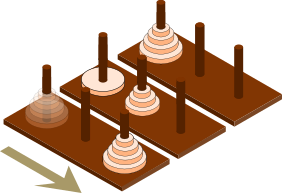
\includegraphics[width=0.7\textwidth]{towers-of-hanoi}
\end{frame}

\begin{frame}[fragile]{Example 4: Recursion can be hard.}
\begin{lstlisting}[mathescape, basicstyle=\scriptsize\ttfamily]
void hanoi(int n, char source, char dest, char spare) { // Function-call cost
  if (n > 0) {                                     // Cost: $\color{codeComment}c_1$
    hanoi(n-1, source, spare, dest);               // Cost: $\color{codeComment}c_2$
    cout << "Move top disk from pole " << source
      << " to pole " << dest << endl;              // Cost: $\color{codeComment}c_3$
    hanoi(n-1, spare, dest, source);               // Cost: $\color{codeComment}c_4$
  }
}
\end{lstlisting}
\begin{itemize}
\item By now, I hope you see that constant and coefficient costs are virtually superfluous when working with Big \(O\).
\item To find the growth-rate function for a recursive algorithm, we have to solve its recurrence relation.
\item You will learn how to do this in Discrete Math.
\end{itemize}
\end{frame}


\begin{frame}{Example 4 continued}
What is the cost of \lstinline{hanoi(n, 'A', 'B', 'C')}?
\begin{itemize}
\item When \(n=0\),
     \( T(0) = c_1 \)
\item When \(n>0\),\\
      \(T(n) = c_1 + c_2 + T(n-1) + c_3 + c_4 + T(n-1)\) \\
           = \(2 \cdot T(n-1) + (c_1+c_2+c_3+c_4)\) \\
           = \(2 \cdot T(n-1) + c \) \textrightarrow{} recurrence equation for the growth-rate function of hanoi-towers algorithm. \\
\item Now, we have to solve this recurrence equation to find the growth-rate function of the hanoi-towers algorithm.
\item This turns out to be \(O(2^n)\) because for every \(n\) we make \(2(n-1)\) calls.
\end{itemize}
\end{frame}


\begin{frame}[fragile]{Example 5: \(O(\)\alt<2->{\(n\)}{?}\()\)}
\begin{lstlisting}[]
int bigOExample5(const int N) {
  const int M = 4 * N;
  int res = 0;
  
  int *pArray = new int[M] {};
  for(int i = 0; i < M; i++) {
    m_pArray[i] = i;
  }
  for(int i = 0; i < M; i++) {
    res += m_pArray[i];
  }
  delete[] pArray;
  return res;
}
\end{lstlisting}
%\(O(\)\alt<2->{\(n\)}{?}\()\)
\onslide<2>{}
\end{frame}

\begin{frame}[fragile]{Example 6: \(O(\)\alt<2->{\(n\)}{?}\()\)}
\begin{lstlisting}[]
int bigOExample6(int n) {
  int total = 0;
  for(int i = 0; i < 4 * n; i++) {
    total += i;
    for(int j = 0; j < 4; j++) {
      total += j;
    }
  }

  return total;
}
\end{lstlisting}
\onslide<2>{}
\end{frame}

\begin{frame}[fragile]{Example 7: \(O(\)\alt<2->{\(n \log{n}\)}{?}\()\)}
\begin{lstlisting}[]
int bigOExample7(int n) {
  int total = 0;
  for(int i = 0; i < n; i++) {
    for(int j = 1; j <= n; j *= 2) {
      total += j;
    }
  }

  return total;
}
\end{lstlisting}
\onslide<2>{}
\end{frame}

%http://academic.regis.edu/dbahr/GeneralPages/DataStructures/DataStrucPart4.pdf

%\section{gprof}
%
%
%\begin{frame}{What is Profiling}
%\begin{itemize}
%\item Allows you to learn:
%\begin{itemize}
%\item where your program is spending its time
%\item what functions called what other functions
%\end{itemize}
%
%\item Can show you which pieces of your program are slower than you expected and might be candidates for rewriting
%
%\item Are functions being called more or less often than expected? 
%
%\item This may help you spot bugs that had otherwise been unnoticed
%\end{itemize}
%\end{frame}
%
%
%\begin{frame}{Profilier}
%\begin{itemize}
%\item It uses information collected during the actual execution of a program
%\item Can be used on programs that are too large or too complex to analyze by reading the source (or you are lazy.)
%\item How your program is run affects the information that shows up in the profile data
%\end{itemize}
%\end{frame}
%
%
%\begin{frame}{Profilier Steps}
%\begin{itemize}
%\item Compile and link your program with profiling enabled
%\item Often this is done by ``-pg'' option
%\item \$ gcc -Wall sampleCode.c -o sampleCode -pg
%\item Execute your program to generate a profile data file
%\item One important point to remember is that the program execution should happen in such a way that all the code blocks (or at least the ones you want to profile) get executed.
%\item \$ ./sampleCode
%\end{itemize}
%\end{frame}
%
%\begin{frame}{Profilier Steps Continued}
%\begin{itemize}
%\item Once the program is executed, it produces a file named gmon.out.
%\item This file contains the profiling data of the code blocks that were actually hit during the program execution. 
%\item It is not a regular text file and therefore cannot be read normally.
%\end{itemize}
%\end{frame}
%
%
%\begin{frame}{Profilier Steps Continued}
%\begin{itemize}
%\item Execute gprof
%\item Once the profiling data (gmon.out) is available, the gprof tool can be used to analyse and produce meaningful data from it.
%\item \$ gprof <command-line-options> <executable-file-name> <profiling-data-file-name> > <output-file>
%\item \$ gprof sampleCode gmon.out > prof\_output
%\end{itemize}
%\end{frame}
%
%
%\begin{frame}{Example}
%\begin{columns}
%\column{0.50\textwidth}
%\includegraphics[width=1.0\textwidth]{prof1.png}
%\column{0.50\textwidth}
%\includegraphics[width=1.0\textwidth]{prof2.png}
%\end{columns}
%\end{frame}
%
%
%\begin{frame}{Flat Profile}
%\begin{itemize}
%\item time your program spent in each function
%\item how many times that function was called 
%\item information on which functions burn most of the cycles is clearly indicated here
%\end{itemize}
%\end{frame}
%
%
%\begin{frame}{Flat Profile Results}
%\includegraphics[width=1.0\textwidth]{prof3.png}
%\begin{itemize}
%\item \textbf{\% time} percentage of the total execution time program spent in this function \\
%all functions combined should add up to 100\%!
%\item \textbf{cumulative seconds}
%This is the cumulative total number of seconds  spent executing this function plus the time spent in all the functions above this one in this table
%\item \textbf{self seconds}
%number of seconds accounted for by this function alone  
%\item flat profile listing is sorted first by this number
%\end{itemize}
%\end{frame}
%
%
%\begin{frame}{}
%\includegraphics[width=1.0\textwidth]{prof3.png}
%\begin{itemize}
%\item \textbf{calls}
%total number of times the function was called 
%if the function was never called, or the number of times it was called cannot be determined (probably because the function was not compiled with profiling enabled), the calls field is blank
%
%\item \textbf{self ms/call}
%represents the average number of milliseconds spent in this function per call
%if this function is not profiled this field is blank 
%
%\item \textbf{total ms/call}
%represents the average number of milliseconds spent in this function and its descendants per call
%if this function is not profiled this field is blank
%\end{itemize}
%\end{frame}
%
%
%\begin{frame}{Call Graph}
%\begin{itemize}
%\item shows, for each function: 
%\item which functions called it, 
%\item which other functions it called,  
%\item how many times it was called. 
%
%\item an estimate of how much time was spent in the subroutines of each function 
%
%\item suggests places where you might try to eliminate function calls that use a lot of time.
%\end{itemize}
%\end{frame}
%
%\begin{frame}{Call Graph}
%\includegraphics[width=1.0\textwidth]{prof4.png}
%\end{frame}
%
%\begin{frame}{Limitations}
%\begin{itemize}

%\item profiling is taken at fixed intervals of run time (so count may be different between runs!)
%\item numerous events may throw off your analysis from actual experiments:
%\begin{itemize}
%\item Varying processor speeds
%\item Varying memory systems (Caches, L1, L2, Main)
%\item Disk speeds \& Network Traffic(I/O operations)
%\item Software instrumentations (what type of optimizations did you uses?)
%\item Computer load during runs
%\end{itemize}
%\item These are beyond the scope fo this class.
%\item Be aware that gprof may give anomalous results (and be ready for them).
%\item Like Newtonian Physics, gprof can be a good approximation.
%\end{itemize}
%\end{frame}



\section{Measuring Time}

%\begin{frame}{Perf}
%\begin{itemize}
%\item Tool to find what part of the code is running slow.
%\item Steps:
%\begin{enumerate}
%\item compile with debug flags! (-g)
%\item run: \\
%%\$ sudo perf record --call-graph dwarf <your-programs-name>
%\$ sudo perf record <your-programs-name>
%\item view the report:\\
%\$ sudo perf report
%\end{enumerate}
%\item Now you should see what functions are taking up all the time!
%\end{itemize}
%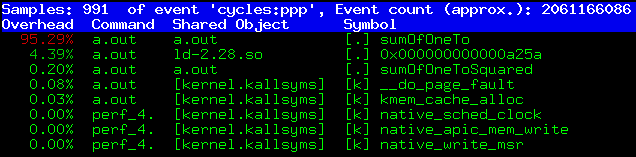
\includegraphics[width=1.0\textwidth]{perf.png}
%\end{frame}


\begin{frame}{Empirical Measurement}
\begin{itemize}
\item While \emph{analytical} performance measures are\\ important, an empirical approach is also insightful.
\item The naive way to take timings:
\begin{enumerate}
\item Record the start time.
\item Run section of code you wish to time.
\item Record the end time.
\item Your answer is (end -- start).
\end{enumerate}
\item While there are numerous issues with this approach, it will give sufficient approximate timings for this class.
\end{itemize}
\end{frame}


\begin{frame}[fragile]{}
\begin{lstlisting}[basicstyle=\scriptsize\ttfamily]
#include <iostream> // To display information
#include <chrono>   // Required for taking timings

void checkTime(const unsigned int MIN_N, const unsigned int MAX_N, const unsigned int CHANGE_IN_N) {
	using namespace std::chrono;
	using clock = std::chrono::steady_clock; // type alias to easily change clock types

	// We want to run our algorithm over varying sizes.
	for (unsigned int size = MIN_N; size <= MAX_N; size += CHANGE_IN_N){
		// Capture the start clock (stored as clock_t)
		const auto START_TIME = clock::now();

		// To Do: This is where your algorithm should be called.
		// Note: size is the SIZE or the input; you may have to change it.
		// functionCallToYouAlgorithm(size);

		// Capture the clock and subtract the start to get the total time elapsed.
		const std::chrono::duration<double> ELAPSED = clock::now() - START_TIME;

		// Convert into seconds as a floating point number.
		const auto TIME_IN_SECS = ELAPSED.count();

		// Print out first the size (size) and then the elapsed time.
		std::cout << size << '\t' << TIME_IN_SECS << '\n';
	}
}
\end{lstlisting}
\end{frame}


\begin{frame}[fragile]{Example Output}

First is the size (1000) and second is the number of seconds (pretty small).

\begin{lstlisting}[basicstyle=\scriptsize\ttfamily\bfseries,identifierstyle=\color{white}, firstnumber=5, firstline=5]
1000	1.711e-06
2000	3.139e-06
3000	4.802e-06
4000	6.423e-06
5000	7.835e-06
6000	9.637e-06
7000	1.0264e-05
8000	1.1698e-05
9000	1.4457e-05
10000	1.5668e-05
11000	1.6472e-05
12000	1.9292e-05
13000	2.0971e-05
14000	1.857e-05
15000	2.124e-05
16000	2.5269e-05
17000	2.4437e-05
18000	2.6614e-05
19000	2.5403e-05
20000	3.0695e-05
\end{lstlisting}
\end{frame}


\section{Gnuplot}

\begin{frame}{Crash Course in gnuplot}

\href{http://www.gnuplot.info/}{\bfseries\texttt{gnuplot}} is an interactive plotting program.

\begin{columns}
\column{0.6\textwidth}
  \begin{itemize}
    \item
      To install, type:\\
      \lstinline[language=bash]{sudo apt update && sudo apt install gnuplot -y}

    \item
      To run, type: \texttt{\textbf{gnuplot}}
  \end{itemize}
\column{0.4\textwidth}

\setbeamercolor{block body}{bg=CSUblue, fg=black}
\begin{block}{\href{https://www.soukoreff.com/gnuplot/}{\small{Higher-Order Knot in gnuplot}}}
\centering
  % 
\includegraphics[width=1.05\textwidth,trim={0 10mm 0 38mm},clip]{gnuplot-example-knot}
  
\includegraphics[width=\textwidth]{gnuplot-example-knot}
\end{block}
\end{columns}
\end{frame}

% \begin{frame}{gnuplot in WSL (Windows System for Linux)}
% To run graphical programs in WSL, we need to run an X-Server in Windows and connect to it.

% For the latest version of WSL, this just works out of the box. However, if you run into problems with an older install, try this manual setup.
% \begin{enumerate}[<+->]
%   \item
%     In Windows, download and install \href{https://sourceforge.net/projects/vcxsrv/}{VcXsrv} as our X-Server.
%   \item
%     In the Windows command line, launch VcXser with the following options.\\
%     \texttt{\bfseries "C:\textbackslash{}Program Files\textbackslash{}VcXsrv\textbackslash{}vcxsrv.exe" :0 -ac -terminate -lesspointer -multiwindow -clipboard -wgl -dpi auto}\\
%     You may wish to create a new shortcut to save these options.
%   \item
%     In an \textbf{admin} command prompt, confirm VxCsrv is running.\\
%     \lstinline{netstat -abno|findstr 6000}
% \end{enumerate}

% \end{frame}


% \begin{frame}{gnuplot in WSL (Windows System for Linux)}
% \begin{enumerate}\setcounter{enumi}{3}
%   \item
%     In Windows, check what version of WSL you are running.\\
%     \lstinline{wsl -l -v}
%   \item <2->
%     In Ubuntu, set the DISPLAY variable.\\
%     \begin{itemize}
%       \item For WSL 2,\\
%         \lstinline[language=Bash]{export DISPLAY=$(cat /etc/resolv.conf | grep nameserver | awk '\{print $2\}'):0}
%       \item For WSL 1,\\
%         \lstinline[language=Bash]{export DISPLAY=:0}
%     \end{itemize}

%   \item <3->
%     To save the DISPLAY configuration for the future, add it to \texttt{\bfseries\textasciitilde/.bashrc}.\\
%       \texttt{\bfseries{}echo "export DISPLAY=\$\{DISPLAY\}" >{}> \textasciitilde/.bashrc}

%   \item  <4->
%     Run \lstinline{gnuplot}.\\
%     If you close VcXsrv, use the shortcut you created to relaunch.
% \end{enumerate}
% \end{frame}

\begin{frame}{Basic Example}
\begin{columns}
\column{0.5\textwidth}

Try typing the following commands:\\
\begin{itemize}
  \item Open gnuplot: \lstinline{gnuplot} \\
  \item Display a sine wave: \lstinline[keepspaces]{plot sin(x) with line}\\
  \item Change from a line to points: \lstinline[keepspaces]{plot sin(x) with point}\\
\end{itemize}

\column{0.5\textwidth}
\setbeamercolor{block body}{bg=white, fg=black}
\begin{block}{gnuplot of sin(x)}
\centering
  
\includegraphics[width=1\textwidth]{gnuplot-sin-line}
\end{block}
\end{columns}
\end{frame}


\begin{frame}[fragile]{Add Labels to the Plot}

Type the following to label your plot.\\
\begin{lstlisting}[language=Bash, basicstyle=\footnotesize\ttfamily]
set title "Sin Wave"           # Add a title to the top.
set ylabel "Amplitude"         # Label the y axis.
set xlabel "Time (in Seconds)" # Label the x axis.
replot                         # Show these changes.
\end{lstlisting}

\setbeamercolor{block body}{bg=white, fg=black}
\setlength{\textwidth}{0.5\textwidth}
\begin{block}{\small{}gnuplot of sin(x) with title and labels}
\centering

\includegraphics[width=1\textwidth]{gnuplot-sin-line-labeled}
\end{block}
\end{frame}


\begin{frame}{Save a Plot to File}
To output the plot to a PDF instead of the screen:\\
\begin{itemize}
  \item \lstinline[language=Bash]{set terminal pdf color}\\
    \lstinline[language=Bash]{set output "nameofplot.pdf"}\\
  \item Then type the commands to plot your data.\\
  \item To save an already-created plot, add \lstinline{replot} or \lstinline{rep}
    to re-plot it in the new output (PDF) device.\\
  \item The data will be written when you exit gnuplot.\\\lstinline[language=Bash]{exit}\\
\end{itemize}

To save the current plot to a file.\\
\begin{itemize}
  \item\lstinline{save "plotname.pdf"}
\end{itemize}
\end{frame}

\begin{frame}{Opening PDF files in VSCodium}
\begin{itemize}
  \item
    For convince, I recommend installing a PDF viewer extension to Visual Studio Code like \href{https://marketplace.visualstudio.com/items?itemName=tomoki1207.pdf}{vscode-pdf}.
  \item
    If you are using the Windows Subsystem for Linux (WSL), also install the \href{https://marketplace.visualstudio.com/items?itemName=ms-vscode-remote.remote-wsl}{WSL extension} by Microsoft. After that, you should see a green box in the bottom left saying ``WSL:Ubuntu''.
  \item
    The following examples assume you can open PDFs in Visual Studio Code.
\end{itemize}
\end{frame}

\begin{frame}[fragile]{Huge Time Saver!}
\texttt{gnuplot} commands can be saved to a script file and automatically used.
\begin{itemize}
\item Create a file named simple.plot containing the following:\\
  \begin{lstlisting}[language=Bash, basicstyle=\small\bfseries\ttfamily]
set terminal pdf color
set output "simple.pdf"
set ylabel "Time (seconds)"
set xlabel "Size"
# Add additional commands...
\end{lstlisting}
\item Run your script and display the PDF: \lstinline{gnuplot simple.plot && code simple.pdf}
\end{itemize}
\end{frame}

\begin{frame}[fragile]{Huge Time Saver!}
Using a gnuplot script is especially useful if you put it in a makefile!

\begin{lstlisting}[language=Make]
plot:
  gnuplot simple.plot # Run gnuplot script
  code simple.pdf # Open the PDF is Visual Studio Code
\end{lstlisting}

Now, \lstinline{make plot} generates the plot and displays it!
\end{frame}

\section{Plotting Timings}

\begin{frame}{Plotting}

\begin{itemize}
\item Assume we have the full listing of performance \\data in a file named \lstinline{single-timings.data}.
\item With gnuplot we can simply graph the timings: \\
\lstinline[keepspaces, language=Bash]{plot "single-timings.data" using 1:2 with line}
\end{itemize}
% \begin{columns}
%   \column{0.5\textwidth}
% \column{0.5\textwidth}
% \setbeamercolor{block body}{bg=white, fg=black}
\begin{center}

% \begin{beamercolorbox}{frametitle}
\fcolorbox{white}{white}{
  
\includegraphics[width=0.55\textwidth]{gnuplot-timings1}
}
% \end{beamercolorbox}
\end{center}
% \end{columns}
\end{frame}

\begin{frame}[fragile]{Automate Testings with a Makefile}
\begin{lstlisting}[basicstyle=\small\ttfamily,language=Make]
.PHONY: plot
all: data.pdf

main: timing-example.cpp
  g++ -Wall -Wextra timing-example.cpp -o main

data.out: main
  ./main > data.out

data.pdf: data.out data.plot
  gnuplot data.plot
  codium data.pdf # Open PDF in VS codium (extension required)

plot: data.pdf
\end{lstlisting}
\end{frame}


\begin{frame}[fragile]{Plotting Multiple Lines from Multiple Files}
  Let us assume we have two files (in the same format),\\ each with timing data for a different algorithm.
\begin{columns}
\column{0.6\textwidth}
\begin{itemize}
\item With gnuplot, we can graph both: \\
\begin{lstlisting}[language=Bash, basicstyle=\footnotesize\ttfamily]
plot "algorithm1.data" using 1:2 with line,\
"algorithm2.data" using 1:2 with line
\end{lstlisting}
\item {You can append more and more data files in this manner.}
\end{itemize}
\column{0.4\textwidth}
\centerline{\Colorbox{white}{
\includegraphics[width=1.0\textwidth]{gnuplot-timings2}}}
\end{columns}
\end{frame}

%\section{Tips \& Gotchas}

\begin{frame}{Summary}
\begin{itemize}
\item In review, we can:
\begin{itemize}
\item Analyze an algorithm analytically to predict performance.
\item Profile programs to find what piece of code is the bottleneck.
\item Output \& plot timings to see actual performance.
\end{itemize}
\item We can spend many hours on \textit{performance analysis}.
\item We stick with the basics for this class.
\item I do want to alert you to a couple of things that will help!
\end{itemize}
\end{frame}

\begin{frame}[fragile]{Common Gotcha}
  You only see one of the two algorithms you plotted!\\
\begin{lstlisting}[language=Bash, basicstyle=\footnotesize\ttfamily,breakindent=5mm]
plot "linear1.data" using 1:2 with line lw 4 title "Linear Algorithm",\
  "quad2.data" using 1:2 with line lw 4 title "Quadratic Algorithm"
\end{lstlisting}

\centerline{\includegraphics[page=1, width=.5\textwidth]{gnuplot-timing-gotcha}}%
\end{frame}

\begin{frame}[fragile]{Common Gotcha}
    Check your data and axis. Often it is too small to see.\\
\begin{lstlisting}[language=Bash, basicstyle=\footnotesize\ttfamily,breakindent=5mm]
plot [:][:0.0001] "linear1.data" using 1:2 with line lw 4 title "Linear Algorithm",\
  "quad2.data" using 1:2 with line lw 4 title "Quadratic Algorithm"
\end{lstlisting}

\centerline{\includegraphics[page=2, width=.5\textwidth]{gnuplot-timing-gotcha}}%
\end{frame}

\begin{frame}{Performance Tips}
\begin{itemize}
\item Optimize the correct functions and look for the correct improvements.
\item From our example, \href{https://en.wikipedia.org/wiki/Perf_\%28Linux\%29}{pref} gives the following:\\
%\includegraphics[width=1.0\textwidth]{prof3.png}
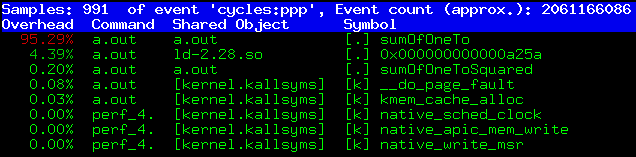
\includegraphics[width=0.8\textwidth]{perf}
\item Most of the time is spent in \lstinline{sumOfOneTo()}; improving \lstinline{sumOfOneTo()}'s performance may help.
\item Optimizing \lstinline{sumOfOneToSquared()} will not help as much.
\begin{itemize}
\item Maybe we can memoize past results to use in the future\\or use a better data structure.
\end{itemize}
\end{itemize}
\end{frame}

\section{Conclusion}



\begin{frame}{Summary}
\begin{itemize}
\item We are scratching the surface.
\item Important outcomes. You should be able to:
\begin{itemize}
\item Analytically deduce the performance of code.
\item Profile code to find the hot spots.
\item Empirically run programs to evaluate performance.
\item Understand that some anomalies will not be addressed in this course.
\end{itemize}
\end{itemize}
\end{frame}

\section*{Lab 7}
\begin{frame}{Lab 7: Performance Analysis}
\centering\Large
Let's take a look at Lab 7.
\end{frame}

\end{document}
